% This section gives an overview of the use cases which are intended for the finished application, most of which will be implemented in this thesis. 
% This section separates the user stories into two subsection "The Launcher" and "The Surveyor", where "The Surveyor stories" was all implemented, while
% "The Launcher stories" where skipped because of time concerns, and to give more time to prioritize "The Surveyor stories".

% \subsubsection{The Launcher}
% \textit{Note that the Launcher was not implemented as part of the thesis.}
% The Launcher should show up when the application is launched and in many ways function as a "server browser".
% Here the user can decide between hosting a session on a 3D model he or she has access to, or join an existing session from a list/browser.
% When the user wishes to initiate or join a session with a particular 3D model to be inspected, he/she should be able to:
% 
% \paragraph{When hosting}a session, the user should be able to:
% \begin{itemize}
% 	\item Specify a 3D model from a standard file format to host the session on.
% 	\item Give the session a name
% 	\item Define a password, which will be required to enter the session. 
% 	\item Choose between different visibility settings for the session (e.g~whether it should show up in the session list)
% \end{itemize}
% 
% \paragraph{When joining}a session, the user  should be able to:
% \begin{itemize}
% 	\item Choose a session from the session list and click the join-button to enter.
% 	\item Enter the name of a session in the search text field to search for a session by name.
% 			This should also enable to find sessions that are otherwise "hidden".
% \end{itemize}	

% Mockup for the launcher?

This section gives an overview of the application functionality, which will be implemented in this thesis.
Initially the design also contained specification for a \textit{launcher program} - a program that orchestrated sessions and provided the boot arguments to the graphical inspector, 
i.e the design review program itself.
In this launcher program a user would be able to either host a design review session by selecting one or multiple 3D models(s) and invite other users, or
join a session by either accepting an invite or browse through available sessions. Because of time concerns, and to give more time to prioritize the 
more thesis-relevant use cases, this functionality was cut and the application instead boots up with tanker model, briefly mentioned in the previous chapter. 

Once the user is loaded into this model, he or she should be able to do the following:
% \subsubsection{The Surveyor}
%Once a user has either created or joined a session and is loaded into the model, he or she should be able to do the following:

\paragraph{Choose between Virtual Reality Mode and Desktop Mode.} Virtual reality mode is meant to be used with a virtual reality headset
and sets up the correct settings (e.g the field of view). Desktop mode is meant to be used without a virtual reality headset and instead used
a regular display. This mode sets up the best setting for regular display usage, and if a virtual reality headset is attached the input from it will be ignored 
(to e.g.~avoid its orientation affecting the camera in the application).

\paragraph{Look around.} When looking around the camera should rotate to the desired direction, but the virtual representation of the user should still keep its orientation. 
This means that the forward direction - the direction the user's body is facing - is the same direction regardless of where the user is looking. 
Looking around should only be achievable when using a virtual reality
headset and having the application in Virtual Reality Mode - as this functionality arguably doesn't have the same applicability in desktop mode. 
If the user is wearing a virtual reality headset, s/he might look around by turning his or her head, so that the VR headset itself also changes orientation.

\paragraph{Rotate (i.e change orientation).} When rotating the whole user should rotate in the desired direction 
(e.g.~The forward-direction changes after a rotation and is where the user is facing after the rotation).
Rotation should allow pitching and yawing (i.e rotation along the Y and Z axis) - the equivalent of looking up and down and from left to right -, 
but not rolling (rotation along the X axis) - the equivalent of doing a "barrel roll" in a jet plane. 
This is because it might cause the user discomfort, specially when using a virtual reality headset, as it is a (arguably) more unnatural movement than the former, and 
has (presumably) little to no practical implications. Rotation should be possible either by using a gesture or by moving the mouse.
% See ~\vref{fig:the_six_degrees_of_freedom} for an illustration.


\paragraph{Move (i.e change position).} The user should be able to move freely along the X, Y and Z axis, and thus be able to move left, right, up, down, forward and backward. 
This movement should happen without regard for any external forces, such as gravity or collision. The user should be able to move by using the keyboard or 
by using gestures. On the keyboard six different keys should be used (forward, backwards, left, right, up and down), while the same should be accomplished by
either three distinct gestures (forward/backward, left/right, up/down) or one combined gesture (forward/backwards/left/right/up/down).

\begin{figure}%[h!] %[H]
	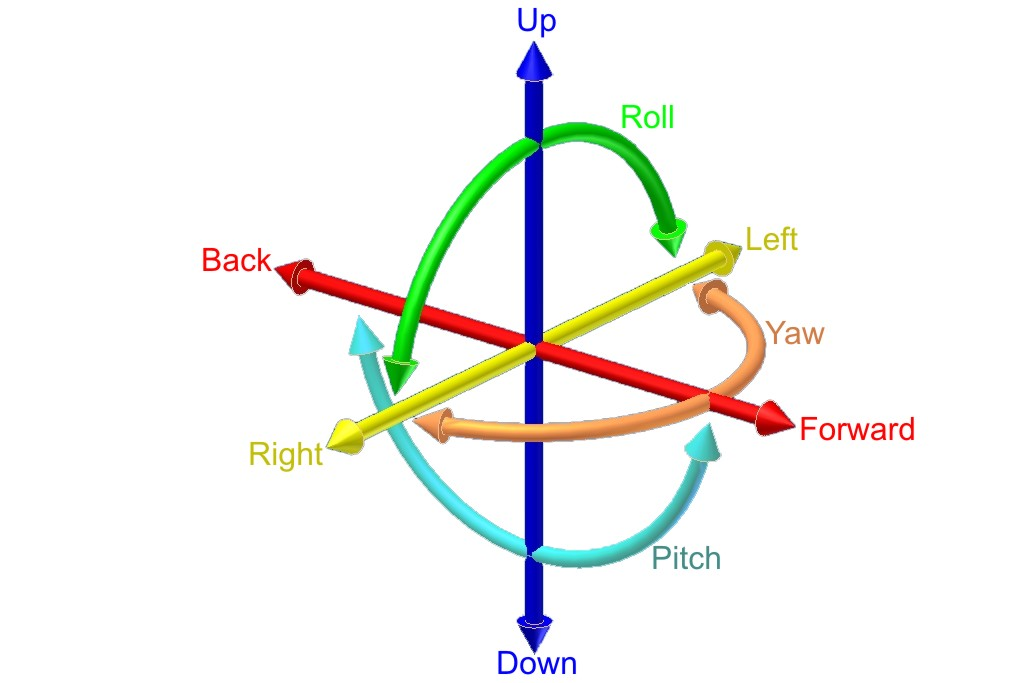
\includegraphics[width=\linewidth]{pictures/the_six_degrees_of_freedom.jpg}
	\caption[The six degrees of freedom]{The six degrees of movement in a three-dimensional space. A rigid body in this space can change position along the X axis (left/right), 
	Y axis (up/down)and Z axis (forward/backward), or change rotation/orientation along the X axis (rolling), Y axis (pitching) and Z axis (yawing).
	Picture from \citet{6DOF}}
	\label{fig:the_six_degrees_of_freedom}
\end{figure} 

\paragraph{Annotate a point (i.e~create a point annotation).} The user should be able to create an annotation - a unit of information related to an aspect of the 3D model - 
and attach it to a surface in the 3D model. 
These annotations can visually be represented as a sphere or orb in the model (to make it uniformly visible from all angles). This should be accomplished by
either clicking the mouse or using a gesture. 

\paragraph{Annotate an object (i.e~create an object annotation).} The user should also be able to annotate a whole object in the 3D model, as opposed to only annotating a point (as in the previous use case). 
When an object, such as a wall, pipe or gear, is annotated in this fashion it should be highlighted or marked by a color in some distinct manner. 
Even though a point annotation - as described in the previous use case - creates an new object in the model (i.e a 3D representation of the annotation), 
an object annotation (as described here) only colors or highlights the object being annotated. 
This should be accomplished by either clicking the mouse or using a gesture. 

\paragraph{Edit an annotation.} The user should be able edit an annotation, either a point or an object annotation, by clicking on the annotation. 
This should bring up a form, which should at least offer the following functionality:
\begin{itemize}
	\item Textual input through a text box.
	\item A submit-button to save the current annotation state and close the annotation form.
	\item A cancel-button to close the annotation form without saving any changes.
	\item A delete-button to delete the annotation, i.e removing the annotation sphere or highlighting and all its associated information. 
	\item Choosing between several annotation categories, labels or states by clicking on one of several associated buttons. 
			These should function as radio-buttons, i.e when one is selected the others are always deselected.
			These categories could refer to the progress status of the task the annotation represents, e.g.~"unresolved", "work in progress" and "approved",
			or they could represent the nature of the annotation itself, e.g.~ "information", "warning" and "error".

	\item A virtual keyboard that can be used instead of the physical keyboard to input text. This is primarily included so the user can input text using 
			gesture recognition technology.
\end{itemize}

\paragraph{Access a menu.} The user should be able to access a menu that offers different options related to the usage of the application.
The menu should allow the the user to:
\begin{itemize}
	\item Go back to the origin position, e.g move and rotate to the same position and orientation as when the application was started.
	\item Choose whether the annotation spheres should be globally visible (e.g.~visible through walls), only visible with line-of-sight or invisible.
		  The first of these options is there to ensure that the user easily can see every annotation, regardless of where the user is in the model,
		  while the other options are there for preference. The default should be global visibility.
	\item Toggle between (i.e turn off or turn on) gesture recognition based on whether it's already turn on or off.
		  This is to enable the user to use his or her hands without it having effect on the application. 
	\item Toggle between having X, Y, and Z axis movement as three separate gestures (forward/backward, left/right, up/down) or one (forward/backwards/left/right/up/down). 
\end{itemize}